% ------------------------------------------------------------------------------
% TYPO3 Version 10 LTS - What's New (French Version)
%
% @license	Creative Commons BY-NC-SA 3.0
% @link		https://typo3.org/help/documentation/whats-new/
% @language	French
% ------------------------------------------------------------------------------

\section{Framework Form}
\begin{frame}[fragile]
	\frametitle{Framework Form}

	\begin{center}\huge{\color{typo3darkgrey}\textbf{Framework Form}}\end{center}
	\begin{center}\large{\textit{Création et gestion de formulaires rendue plus aisée}}\end{center}

\end{frame}

% ------------------------------------------------------------------------------
% Feature | 79445 | Add Multistep Wizard

\begin{frame}[fragile]
	\frametitle{Framework Form}
	\framesubtitle{Assistant multi-étapes}

	\begin{itemize}
		\item Le module JavaScript \texttt{MultiStepWizard} est introduit,
			ajoutant les fonctionnalités suivantes~:

			\begin{itemize}
				\item Navigation vers l'étape précédente.
				\item Libellés descriptifs tel que «~Début~» ou «~Fin~», au lieu de l'indicateur numérique «~Étape x de y~».
				\item Structure de configuration optimisée.
			\end{itemize}

		\item Voir le \href{https://docs.typo3.org/c/typo3/cms-core/master/en-us/Changelog/10.2/Feature-79445-AddMultistepWizard.html}{journal des changements (en)}
			pour des exemples de code JavaScript.

		\item Cette fonctionnalité améliore significativement l'expérience utilisateur~: les utilisateurs backend remarquerons
			un assistant de création de formulaire amélioré.

	\end{itemize}

\end{frame}

% ------------------------------------------------------------------------------
% Feature | 84757 | Double click in structure tree changes label

\begin{frame}[fragile]
	\frametitle{Backend User Interface}
	\framesubtitle{Édition des titres}

	Les libellés des champs de formulaire sont éditables en double-cliquant directement sur le titre dans l'arborescence.

	\begin{figure}
		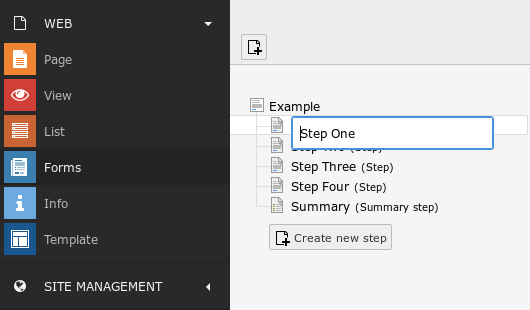
\includegraphics[width=0.5\linewidth]{FormFramework/84757-DoubleClickToChangeLabel.png}
	\end{figure}

\end{frame}

% ------------------------------------------------------------------------------
% Important | 84221 | Restructuring of form setup

\begin{frame}[fragile]
	\frametitle{Framework Form}
	\framesubtitle{Configuration du formulaire}

	\begin{itemize}
		\item Trois fichiers étaient utilisés~: \texttt{BaseSetup.yaml}, \texttt{FormEditorSetup.yaml}, et \texttt{FormEngineSetup.yaml}.
		\item Ils sont rationalisés et consolidés dans un seul fichier~: \texttt{FormSetup.yaml}.
		\item Ce fichier contient la configuration de base, incluant les importations de configuration pour les validateurs,
			les éléments de formulaire et les finaliseurs.
		\item Tous les héritages et incorporations (mixin) sont résolues, rendant la compréhension de la configuration plus aisée.
	\end{itemize}

\end{frame}

% ------------------------------------------------------------------------------
% Breaking | 87009 | Use multiple translation files by default in EXT:form

\begin{frame}[fragile]
	\frametitle{Framework Form}
	\framesubtitle{Traductions}

	% decrease font size for code listing
	\lstset{basicstyle=\tiny\ttfamily}

	\begin{itemize}
		\item L'option suivante est renommée~:\newline
			\small\texttt{translationFile} \textrightarrow\hspace{0.1cm}\texttt{translationFiles}\normalsize
		\item Les fichiers de traduction par défaut sont déclarés en index 10~:

			\begin{itemize}
				\item \texttt{EXT:form/Resources/Private/Language/locallang.xlf}
				\item \texttt{EXT:form/Resources/Private/Language/Database.xlf}
			\end{itemize}

		\item Les formulaires personnalisés en configuration YAML doivent être mis à jour.

\begin{lstlisting}
ANCIEN :
translationFile: path/to/locallang.xlf

NOUVEAU :
translationFiles:
  20: path/to/locallang.xlf
\end{lstlisting}

	\end{itemize}

\end{frame}

% ------------------------------------------------------------------------------
% Feature | 84203 | Unify form setup YAML loading

\begin{frame}[fragile]
	\frametitle{Framework Form}
	\framesubtitle{Fichiers YAML}

	\begin{itemize}
		\item Les fichiers YAML utilisent le chargeur de YAML du noyau de TYPO3.
		\item Ces fonctionnalités sont donc accessibles~:

			\begin{itemize}
				\item Importation de fichiers YAML à l'aide de la directive \texttt{imports}.
				\item Remplacement des \texttt{\%substitutions\%}.
			\end{itemize}

	\end{itemize}

\end{frame}

% ------------------------------------------------------------------------------
% Feature | 90052 | Form YAML configuration available in configuration module

\begin{frame}[fragile]
	\frametitle{Framework Form}
	\framesubtitle{Configuration YAML}

	\begin{columns}[T]
		\begin{column}{.04\textwidth}
		\end{column}
		\begin{column}{.38\textwidth}

			Lorsque l'extension système \texttt{EXT:form} est activée, la configuration YAML chargée
			est disponible sous \textbf{SYSTÈME} $\rightarrow$ \textbf{Configuration}.

			\vspace{0.2cm}

			Ceci nécessite bien sûr que l'extension \texttt{EXT:lowlevel} soit activée.

		\end{column}
		\begin{column}{.58\textwidth}
			\vspace{-0.3cm}
			\begin{figure}
				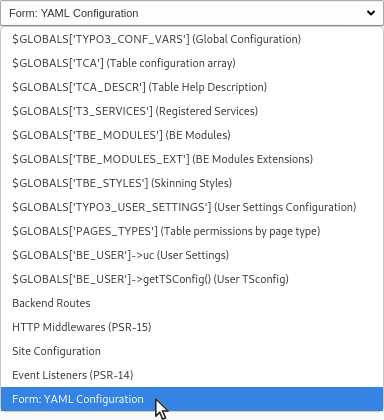
\includegraphics[width=0.70\linewidth]{FormFramework/90052-AddYamlConfigurationToConfigurationModule.png}
			\end{figure}
		\end{column}
	\end{columns}

\end{frame}

% ------------------------------------------------------------------------------
% Feature | 89747 | Custom tables with record browser in forms

\begin{frame}[fragile]
	\frametitle{Framework Form}
	\framesubtitle{Explorateur d'enregistrements (1)}

	% decrease font size for code listing
	\lstset{basicstyle=\tiny\ttfamily}

	\begin{itemize}
		\item L'explorateur d'enregistrements se configure pour utiliser des tables supplémentaires~:
\begin{lstlisting}
TYPO3:
  CMS:
    Form:
      prototypes:
        standard:
          formElementsDefinition:
            MyCustomElement:
              formEditor:
                editors:
                  # ...
                  300:
                    identifier: myRecord
                    # ...
                    browsableType: tx_myext_mytable
                    propertyPath: properties.myRecordUid
                    # ...
\end{lstlisting}

	\end{itemize}

\end{frame}

% ------------------------------------------------------------------------------
% Feature | 89746 | Custom icon for record browser button in forms

\begin{frame}[fragile]
	\frametitle{Framework Form}
	\framesubtitle{Explorateur d'enregistrements (2)}

	% decrease font size for code listing
	\lstset{basicstyle=\tiny\ttfamily}

	\begin{itemize}
		\item L'icône du bouton de l'explorateur d'enregistrements est personnalisable~:
\begin{lstlisting}
TYPO3:
  CMS:
    Form:
      prototypes:
        standard:
          formElementsDefinition:
            MyCustomElement:
              formEditor:
                editors:
                  # ...
                  300:
                    identifier: contentElement
                    # ...
                    browsableType: tt_content
                    iconIdentifier: mimetypes-x-content-text
                    propertyPath: properties.contentElementUid
                    # ...
\end{lstlisting}

	\end{itemize}

\end{frame}

% ------------------------------------------------------------------------------
% Feature | 84713 | Access single values in form templates

\begin{frame}[fragile]
	\frametitle{Framework Form}
	\framesubtitle{Explorateur d'enregistrements (3)}

	% decrease font size for code listing
	\lstset{basicstyle=\tiny\ttfamily}

	\begin{itemize}
		\item Le nouveau \textit{RenderFormValue-ViewHelper} permet aux intégrateurs et développeurs
			d'accéder à une valeur du formulaire dans les gabarits Fluid~:
\begin{lstlisting}
<p>
  The following message was just sent by
  <formvh:renderFormValue renderable="{page.rootForm.elements.name}" as="formValue">
    {formValue.processedValue}
  </formvh:renderFormValue>:
</p>

<blockquote>
  <formvh:renderFormValue renderable="{page.rootForm.elements.message}" as="formValue">
    {formValue.processedValue}
  </formvh:renderFormValue>
</blockquote>
\end{lstlisting}

	\end{itemize}

\end{frame}

% ------------------------------------------------------------------------------
% Feature | 82706 | Render fieldset labels in form templates

\begin{frame}[fragile]
	\frametitle{Framework Form}
	\framesubtitle{Libellé des groupes}

	\begin{itemize}
		\item L'élément de groupe / section \texttt{Fieldset} est disponible dans les gabarits.
		\item Par défaut, sont affectés l'élément de formulaire \textbf{SummaryPage} et les finaliseurs \textbf{EmailToReceiver} et \textbf{EmailToSender}.
		\item Cas d'usage typique~:\newline
			\small
				Un formulaire avec une adresse d'expédition et une de facturation. Les deux sections peuvent avoir des
				champs de même nom, i.e. \texttt{rue}. La distinction de ces champs s'effectue en utilisant le libellé du groupe.
			\normalsize

	\end{itemize}

\end{frame}

% ------------------------------------------------------------------------------
% Deprecation | 88238 | Allowed MIME types of FileUpload and ImageUpload

\begin{frame}[fragile]
	\frametitle{Framework Form}
	\framesubtitle{Chargement de fichiers}

	\begin{itemize}
		\item Les \texttt{allowedMimeTypes} prédéfinis pour les éléments de formulaire
			suivant sont marqués \textbf{dépréciés}~:

			\begin{itemize}
				\item \texttt{FileUpload}
				\item \texttt{ImageUpload}
			\end{itemize}

		\item Tous les types MIME valides doivent être explicitement listés dans le définition du formulaire\newline
			\smaller
				(les types MIME prédéfinis seront retirés de TYPO3 v11)
			\normalsize

	\end{itemize}

\end{frame}

% ------------------------------------------------------------------------------
% Deprecation | 89742 | Form mixins

\begin{frame}[fragile]
	\frametitle{Framework Form}
	\framesubtitle{Incorporation de formulaire}

	\begin{itemize}
		\item Les incorporation (mixins) sont marquées \textbf{dépréciées} et ne devraient plus être utilisées.
		\item Tous les héritage depuis \texttt{TYPO3.CMS.Form.mixins.*} sont affectés.
		\item Options de migration~:

			\begin{itemize}
				\item Intégrer les parties essentielles depuis \texttt{TYPO3.CMS.Form.mixins.*}, ou
				\item les migrer vers des incorporations personnalisées.
			\end{itemize}

	\end{itemize}

\end{frame}

% ------------------------------------------------------------------------------
% Feature | 80420 | Allow multiple recipients in email finisher

\begin{frame}[fragile]
	\frametitle{Framework Form}
	\framesubtitle{Destinataires multiples (1)}

	\begin{itemize}
		\item Les mails envoyés au travers de \textit{EmailFinisher} peuvent avoir de multiples destinataires.

		\item Les options introduites sont~:

			\begin{itemize}
				\item \texttt{recipients} (To)
				\item \texttt{replyToRecipients} (Reply-To)
				\item \texttt{carbonCopyRecipients} (CC)
				\item \texttt{blindCarbonCopyRecipients} (BCC)
			\end{itemize}

	\end{itemize}

\end{frame}

% ------------------------------------------------------------------------------
% Feature | 80420 | Allow multiple recipients in email finisher

\begin{frame}[fragile]
\frametitle{Framework Form}
\framesubtitle{Destinataires multiples (2)}

	% decrease font size for code listing
	\lstset{basicstyle=\tiny\ttfamily}

	\begin{itemize}
		\item Ce changement nécessite la migration manuelle des options valeur simple à leur nouvelle forme~:

		\smaller\textbf{Ancienne} configuration \textit{Finisher}~:\normalsize

\begin{lstlisting}
finishers:
  -
    identifier: EmailToReceiver
    options:
      recipientAddress: utilisateur@example.com
      recipientName: 'Prenom Nom'
\end{lstlisting}

		\smaller\textbf{Nouvelle} configuration \textit{Finisher}~:\normalsize

\begin{lstlisting}
finishers:
  -
    identifier: EmailToReceiver
    options:
      recipients:
        utilisateur@example.com: 'Prenom Nom'
\end{lstlisting}

		\item Voir le \href{https://docs.typo3.org/c/typo3/cms-core/10.0/en-us/Changelog/master/Deprecation-80420-EmailFinisherSingleAddressOptions.html}{journal des changements (en)}
			pour plus d'exemples de migration.

	\end{itemize}

\end{frame}

% ------------------------------------------------------------------------------
% Deprecation | 87200 | EmailFinisher format option
% Deprecation | 87200 | EmailFinisher FORMAT_* constants

\begin{frame}[fragile]
	\frametitle{Framework Form}
	\framesubtitle{Texte brut/HTML}

	\begin{itemize}
		\item Les emails envoyés par \textit{EmailFinisher} peuvent être envoyés en texte brut, HTML ou les deux.

		\item Dans le même temps, l'option \texttt{format} est marquée dépréciée et sera retirée en TYPO3 v11.

		\item Les valeurs existantes seront automatiquement migrées~:

			\begin{itemize}\smaller
				\item \texttt{format:html} \tabto{3cm}\textrightarrow\hspace{0.1cm}\texttt{addHtmlPart:\textbf{true}}
				\item \texttt{format:plaintext} \tabto{3cm}\textrightarrow\hspace{0.1cm}\texttt{addHtmlPart:\textbf{false}}
				\item sans «~\texttt{format}~» \tabto{3cm}\textrightarrow\hspace{0.1cm}\texttt{addHtmlPart:\textbf{true}}
			\end{itemize}\normalsize

		\item Ces deux constantes sont marquées dépréciées~:

			\begin{itemize}\smaller
				\item \texttt{EmailFinisher::FORMAT\_PLAINTEXT}
				\item \texttt{EmailFinisher::FORMAT\_HTML}
			\end{itemize}\normalsize

	\end{itemize}

\end{frame}

% ------------------------------------------------------------------------------
% Feature | 87798 | Provide a way to sort form lists in ext:form

\begin{frame}[fragile]
	\frametitle{In-depth Changes}
	\framesubtitle{Tri des formulaires}

	% decrease font size for code listing
	\lstset{basicstyle=\tiny\ttfamily}

	\begin{itemize}
		\item Les formulaires peuvent être triés en ordre ascendant ou descendant.
		\item Deux options sont introduites~: \texttt{sortByKeys} et \texttt{sortAscending}.
		\item Les formulaires sont triés initialement par leur nom et l'identifiant de leur fichier (ascendant).
		\item Pour changer le tri, la configuration suivante doit être utilisée de la fichier de configuration YAML~:
\begin{lstlisting}
TYPO3:
  CMS:
    Form:
      persistenceManager:
        sortByKeys: ['name', 'fileUid']
        sortAscending: true
\end{lstlisting}

	\end{itemize}

\end{frame}

% ------------------------------------------------------------------------------
